\documentclass{article}
\usepackage{pgfplots}
\usepgfplotslibrary{fillbetween}
\pgfplotsset{compat=1.18}

\begin{document}

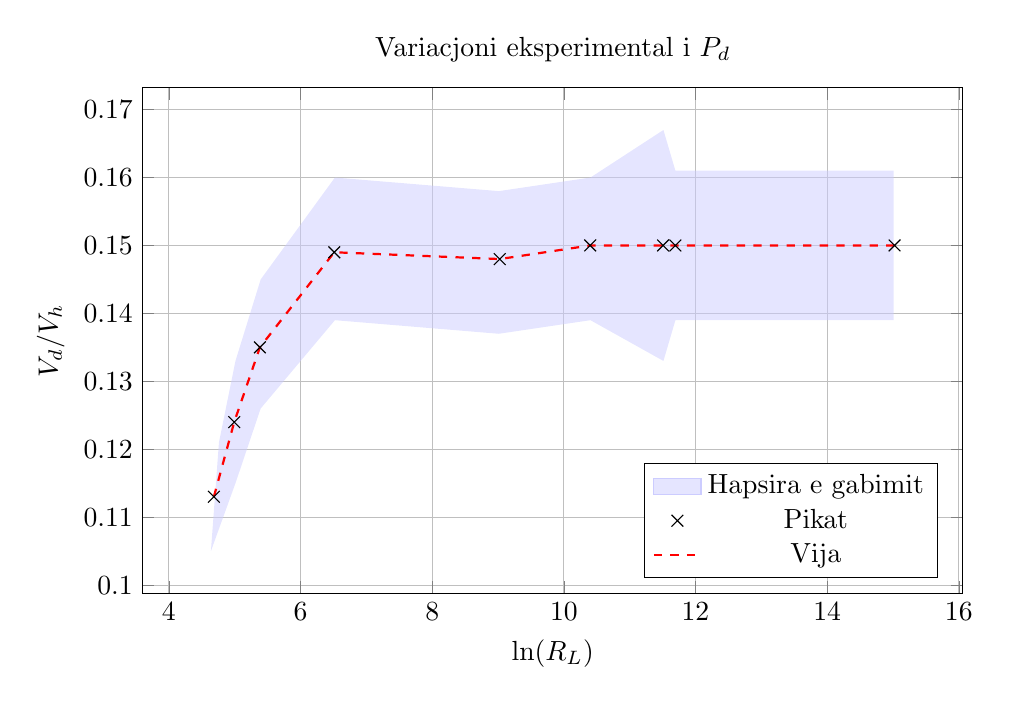
\begin{tikzpicture}
    \begin{axis}[
        xlabel={$\ln(R_L)$},
        ylabel={$V_d/V_h$},
        title={Variacjoni eksperimental i $P_d$ },
        grid=major,
        legend pos=south east,
        width=12cm,
        height=8cm
    ]
    
    %Lower bound
    \addplot[name path=lower, draw=none, forget plot] coordinates {
        (4.638, 0.105)
        (5.011, 0.115)
        (5.394, 0.126)
        (6.522, 0.139)
        (9.012, 0.137)
        (10.404, 0.139)
        (11.513, 0.133)
        (11.695, 0.139)
        (15.009, 0.139)
    };

    %Upper bound
    \addplot[name path=upper, draw=none, forget plot] coordinates {
        (4.760, 0.121)
        (5.011, 0.133)
        (5.394, 0.145)
        (6.522, 0.160)
        (9.012, 0.158)
        (10.404, 0.160)
        (11.513, 0.167)
        (11.695, 0.161)
        (15.009, 0.161)
    };

    %Plot fill
    \addplot[blue!20, fill opacity=0.5] 
        fill between[of=lower and upper];
    \addlegendentry{Hapsira e gabimit}

    %Data points
    \addplot[
        only marks, 
        black, 
        mark=x,
        mark size=3pt,
        mark options={solid}
    ] coordinates {
        (4.683, 0.113)
        (4.992, 0.124)
        (5.382, 0.135)
        (6.512, 0.149)
        (9.026, 0.148)
        (10.401, 0.150)
        (11.507, 0.150)
        (11.695, 0.150)
        (15.024, 0.150)
    };
    \addlegendentry{Pikat}
    
    %Dashed line
    \addplot[red, dashed, thick] coordinates {
        (4.683, 0.113)
        (4.992, 0.124)
        (5.382, 0.135)
        (6.512, 0.149)
        (9.026, 0.148)
        (10.401, 0.150)
        (11.507, 0.150)
        (11.695, 0.150)
        (15.024, 0.150)
    };
    \addlegendentry{Vija}

    \end{axis}
\end{tikzpicture}

\end{document}